\section{Cálculo Vetorial de Curvas}


\begin{definb}{}{}
Uma parametrização {\color{red} $\vec{r}=\vec{r}(t)$} é chamada {\color{blue} suave} em um intervalo $I$ se {\color{red}$\vec{r}\,^\prime$} for contínua e {\color{red}$\vec{r}\,^\prime(t)\neq \vec{0}$} em $I$.
\end{definb}


\marcador{subsection}{Parametrização pelo comprimento de arco}

Seja $C$ uma curva {\color{blue}suave} parametrizada por $\vec{r}=\vec{r}(t)$, $a\leq t\leq b$. Definimos a sua {\color{blue} função comprimento de arco} por
\[s(t)=\int_a^t\|\vec{r}\,^\prime (u)\|du.\]

Note que
\[\frac{ds}{dt}=\|\vec{r}\,^\prime (t)\|> 0,\]
assim $s=s(t)$ é uma {\color{red}função crescente} e de classe $C^1$. Neste caso, $s$ possui uma inversa, denotada por $t=t(s)$.

\vfill

Isso nos permite {\color{red} reparametrizar a curva $C$ em relação ao comprimento de arco} fazendo
\[\vec{r}(s)=\vec{r}(t(s)),\ 0\leq s\leq L,\]
onde $L$ é o comprimento final da curva.

\begin{caixaazul}{}{}
É frequentemente útil usar a parametrização em relação ao comprimento de arco, pois este não depende do sistema de coordenadas nem da parametrização.
\end{caixaazul}
\newpage


\begin{exeb}{}{}
Reparametrize a hélice circular $\vec{r}(t)=(\cos(t),\sin(t),t)$ utilizando o comprimento de arco a partir do ponto $(1,0,0)$.
\end{exeb}
\vfill

\begin{caixaazul}{}{}
Quando a curva está parametrizada pelo comprimento de arco, geometricamente isso significa que o ponto $\vec{r}(s)$  é o ponto da curva que está a $s$ unidades de comprimento do início da curva.
\end{caixaazul}
\newpage

\begin{casab}{}{}
Seja $\vec{r}(t)=(e^t\sin(t),e^t\cos(t),\sqrt{2}e^t)$ e $P=(0,1,\sqrt{2})$.
\begin{enumerate}
\item Encontre a função comprimento de arco da curva medida a partir do ponto $P$ na direção crescente de $t$.
\item Reparametrize a curva com relação ao comprimento de arco começando de $P$.
\item Encontre o ponto a 4 unidades de $P$ ao longo da curva na direção crescente de $t$.
\end{enumerate}
\end{casab}
\newpage

\marcador{subsection}{Curvatura}

Se $C$ é uma curva parametrizada por $\vec{r}=\vec{r}(t)$ suave, então o {\color{blue}vetor tangente unitário} é definido por:
\[\vec{T}(t)=\frac{\vec{r}\,^\prime(t)}{\|\vec{r}\,^\prime(t)\|}.\]



O vetor tangente unitário indica a direção da curva e muda de direção muito devagar quando a curva $C$ é razoavelmente reta, mas muda mais rapidamente quando se dobra mais acentuadamente.

\begin{center}
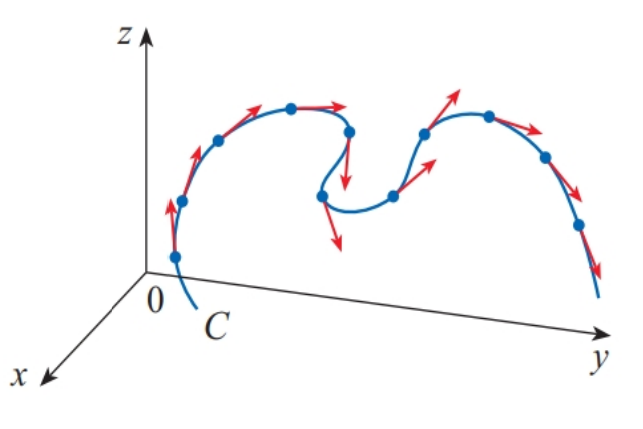
\includegraphics[scale=0.6]{figuras/vetor-tangente.png}
\end{center}
\newpage

A {\color{blue}curvatura} de $C$, em dado ponto, será definida de modo a medir

\begin{caixaazul}{}{}
{A taxa de variação da direção do vetor tangente unitário \textbf{\color{red}por unidade de comprimento}.}
\end{caixaazul}
Em outras palavras,
\begin{caixaazul}{}{}
{A medida de quão rapidamente a curva muda de direção no ponto}.
\end{caixaazul}

Por isso, definimos a curvatura como a norma  da taxa de variação do vetor tangente unitário com relação ao comprimento de arco, a saber,

%\begin{center}
\begin{caixaazul}{Fórmula de definição da Curvatura}{}
Seja $C$ uma curva {\color{blue}suave}, {\color{red}parametrizada pelo comprimento de arco}. A {\color{blue} curvatura } de \(C\) é a função
\[\kappa(s)=\left\|\frac{d\vec{T}(s)}{ds}\right\|\]
onde $\vec{T}$ é o vetor tangente unitário.
\end{caixaazul}


%\end{center}


%\[
%\kappa(s)=\left\|\frac{d\vec{T}(s)}{ds}\right\|,
%\]



\begin{exeb}{}{}
 Determine a curvatura da hélice circular $\vec{r}(t)=(\cos(t),\sin(t),t)$ utilizando a reparametrização pelo comprimento de arco do exemplo anterior.
\end{exeb}
\newpage

Entretanto, na maioria das vezes a curva não está parametrizada pelo comprimento de arco. Neste caso, podemos usar a Regra da Cadeia para obter uma fórmula em termos de um parâmetro qualquer. Se $s=s(t)$ é a função comprimento de arco, então:
\[\frac{d\vec{T}(s(t))}{dt}=\frac{d\vec{T}(s)}{ds}\frac{ds}{dt}=\frac{d\vec{T}}{ds}\|\vec{r}\,^\prime(t)\|.\]
Logo,

\begin{caixaazul}{Fórmula da curvatura para uma parametrização arbitrária}{}
\[\kappa(t)=
\frac{\|\vec{T}\,^\prime(t)\|}{\|\vec{r}\,^\prime(t)\|}
\]
\end{caixaazul}
%\[{\color{red} \kappa(t) =\frac{\|\vec{T}\,^\prime(t)\|}{\|\vec{r}\,^\prime(t)\|}.}\]
\vfill

\begin{exeb}{}{}
\begin{enumerate}[(a)]
\item Calcule a curvatura de um círculo de raio $\rho$.
\item Calcule a curvatura da parábola.
\end{enumerate}

\end{exeb}
\newpage

\marcador{subsection}{Vetores Normal principal e Binormal}


Como $\vec{T}$ é unitário, sabemos que $\vec{T}$ é ortogonal à  $\vec{T}\,^\prime$, portanto definimos o {\color{blue} vetor normal unitário principal} ou simplesmente  {\color{blue} vetor normal unitário} como

\begin{center}
\destaque{
\(\vec{N}(t)=\frac{\vec{T}\,^\prime(t)}{\|\vec{T}\,^\prime(t)\|}\)
}
\end{center}
%\[\color{red} \vec{N}(t)=\frac{\vec{T}\,^\prime(t)}{\|\vec{T}\,^\prime(t)\|}.\]
Este vetor indica a direção que na qual a curva está virando em cada ponto. A partir dele, definimos o {\color{blue} vetor binormal unitário}

\begin{center}
\destaque{
\( \vec{B}(t)=\vec{T}(t)\times \vec{N}(t)\)
}
\end{center}
%\[\color{red} \vec{B}(t)=\vec{T}(t)\times \vec{N}(t).\]

\begin{center}
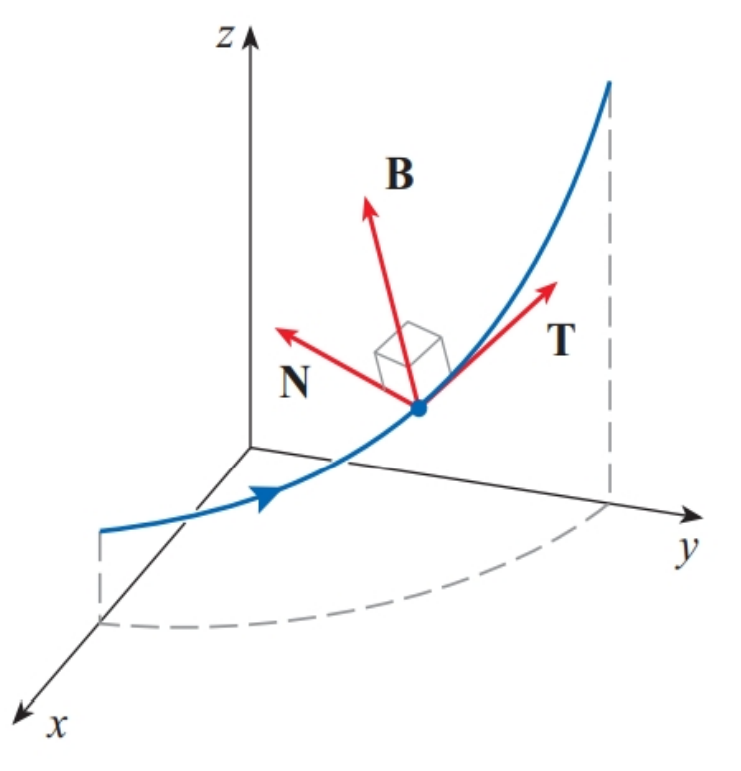
\includegraphics[scale=0.4]{figuras/normal-binormal.png}
\end{center}

Estes três vetores formam uma base ortonormal muito importante em geometria diferencial e no estudo de movimento de corpos, chamada de {\color{blue} Triedro de Frenet}.

\begin{exeb}{}{}
Determine os vetores normal e binormal da hélice circular $$\vec{r}(t)=(\cos(t),\sin(t),t).$$

\end{exeb}

\newpage


\marcador{subsection}{Movimento: velocidade e aceleração}

Suponha que uma partícula se mova de forma que seu vetor posição no instante $t$ seja $\vec{r}(t)$. Então vamos denotar por:
\begin{itemize}
	\item $\vec{v}(t)=\vec{r}\,'(t)$ é o vetor \dt{velocidade da partícula} no instante $t$.
	\item $v(t)=\|\vec{v}(t)\|$ é a \dt{velocidade escalar} da partícula no instante $t$.
	\item $\vec{a}(t)=\vec{r}\,''(t)$ é o vetor \dt{aceleração} da partícula no instante $t$.
	\item $a(t)=\|\vec{a}(t)\|$ a \dt{aceleração escalar} da partícula no instante $t$.
\end{itemize}


Podemos mostrar que  a aceleração é dada por:

\begin{center}
\destaque{
\(\vec{a}={\color{red} v'}\vec{T}+{\color{blue}v^2\kappa} \vec{N}\)
}
\end{center}


%\[{\color{red}\vec{a}=v'\vec{T}+v^2\kappa \vec{N}. }\]

\newpage
Com isso temos as seguintes conclusões:
\begin{itemize}
\item O vetor $\vec{B}$ não aparece, ou seja, a aceleração sempre está no plano determinado por $\vec{T}$ e $\vec{N}$, chamado {\color{blue} plano osculador}.


\item A {\color{red}componente tangencial} da aceleração mede a taxa de variação do módulo da  velocidade, isto é, a {\color{red}mudança na velocidade escalar}.

\item A {\color{blue}componente normal} é dada pelo quadrado da velocidade escalar e pela curvatura.
\end{itemize}

\begin{exeb}{}{}
Um objeto de massa $m$ que se move em uma trajetória circular com velocidade angular constante $\omega$ tem vetor posição dado por $\vec{r}(t)=(\rho\cos (\omega t), \rho\sin (\omega t)).$ Determine a força que age sobre o objeto.
\end{exeb}

\newpage


Usando a última equação, podemos deduzir a seguinte fórmula para a curvatura.
\begin{caixaazul}{Terceira fórmula da curvatura}{}
A curvatura de uma curva parametrizada suave $\vec{r}=\vec{r}(t)$ é dada por:
\[\kappa(t)=\frac{\|\vec{v}(t)\times \vec{a}(t)\|}{v^3(t)}=\frac{\|\vec{r}\,^\prime(t)\times \vec{r}\,^{\prime\prime}(t)\|}{\|\vec{r}\,^\prime(t)\|^3}.\]
\end{caixaazul}
\vfill

\begin{exeb}{}{}
Determine a curvatura da cúbica retorcida $\vec{r}(t)=(t,t^2,t^3)$.
\end{exeb}
\newpage


\begin{casab}{}{}
\begin{enumerate}

\item  Mostre que a curvatura de uma curva plana que tem equação cartesiana da forma $y=f(x)$ é dada por:
\[\kappa(x)=\frac{|f''(x)|}{\left(1+[f'(x)]^2\right)^{3/2}}.\]

\item Calcule a curvatura da parábola $y=x^2$ e determine o ponto onde a curvatura é máxima.

\item Determine as componentes normal e tangencial da aceleração da partícula que se move segundo a trajetória $\vec{r}(t)=e^{-t}\,\vec{i}+e^t\,\vec{j}$.

\item Uma partícula se move sobre a parábola $y=x^2$ da esquerda para a direita. Quando ela passa pelo ponto $(2,4)$, sua velocidade é $v=3$ m/s e $v'=7$ m/s$^2$. Ache o vetor velocidade e o vetor aceleração neste ponto.

\item Determine as componentes tangencial e normal do vetor aceleração da curva
\[\vec{r}(t)=(t^2+1)\vec{i}+t^3\vec{j}, \ t\geq 0.\]


\item Determine uma parametrização para a reta tangente à hélice $\vec{r}(t)=\left(2\cos t,\sin t, t\right)$ no ponto $P=(0,1,\pi/2)$.

\item Determine o comprimento de arco da cardioide $r=2(1+\cos \theta)$.

%\item Determine os vetores velocidade e aceleração e a velocidade escalar da partícula cuja função posição é
%\[\vec{r}(t)=3\cos(t)\,\vec{i}+2\sin( t)\, \vec{j},  0\leq t\leq 2\pi.\]
%Faça um esboço da trajetória e marque os vetores velocidade onde a velocidade escalar é mínima e máxima.
	\end{enumerate}
\end{casab}